\section{Redukovani uredjeni binarni dijagrami odlu\v{c}ivanja (ROBDD)}
\label{sec:OBDD}

Uredjeni binarni dijagrami odlu\v{c}ivanja (engl. \emph{Ordered Binary Decision Diagrams}, u daljem tekstu \emph{OBDD}) su BDD u kojima se promenljive uvek testiraju u istom redosledu. OBDD se naziva \emph{redukovano}(engl. \emph{Reduced Ordered Binary Decision Diagrams} \cite{ROBDD}, u daljem tekstu \emph{ROBDD}) ukoliko ima slede\'c{}e osobine:
\begin{itemize}
    \item Neredundantnost - Visoko i nisko podstablo svakog \v{c}vora je razli\v{c}ito.
    \item Jedinstvenost - Ne postoje dva razli\v{c}ita \v{c}vora koja testiraju istu promenljivu, a \v{c}ija su podstabla ista.
\end{itemize}

Kao \v{s}to je pomenuto u poglavlju \ref{sec:BinarnaDrvetaOdlucivanja}, binarna drveta odlu\v{c}ivanja poseduju osobinu kanoni\v{c}nosti. Medjutim, kako postoje razli\v{c}ita BDD koja odgovaraju jednom binarnom drvetu odlu\v{c}ivanja, jasno je da BDD nemaju ovu osobinu. Uprkos tome, zbog svojih lepih i jasno definisanih osobina, ROBDD je takodje kanoni\v{c}no. Pro\v{s}irivanjem definicije kanoni\v{c}nosti na ROBDD, dobijamo tvrdjenje: kanoni\v{c}nost ROBDD zna\v{c}i da za fiksan redosled promenljivih, svaka bulovska funkcija ima jedinstvenu reprezentaciju u vidu ROBDD. Ovo zna\v{c}i da mo\v{z}emo uporediti bulovske funkcije konstrukcijom njihovih ROBDD, a ukoliko su ona jednaka, to garantuje njihovu ekvivalentnost.

ROBDD ima najvi\v{s}e dva lista: 0 i 1. U nastavku \'c{}emo ponekad crtati oba, kako bi se smanjila kompleksnost njhovog grafi\v{c}kog prikaza.



\subsection{Konstrukcija ROBDD}
\label{subsec:ROBDDConstruction}

ROBDD se mo\v{z}e konstruisati na vi\v{s}e na\v{c}ina. U ovom poglavlju \'c{}e najpre \'c{}e biti opisana naivna metoda konstrukcije (videti \ref{subsubsec:naiveROBDDConstruction}), a zatim \'c{}e ukratko biti opisana efikasnija metoda (videti \ref{subsubsec:optimalROBDDConstruction}).


\subsubsection{Naivna konstrukcija ROBDD}
\label{subsubsec:naiveROBDDConstruction}

Najjednostavniji na\v{c}in da se konstrui\v{s}e ROBDD je da se najpre konstrui\v{s}e ekvivalentno uredjeno binarno drvo odlu\v{c}ivanja. Nakon toga se primenjuju slede\'c{}a pravila dokle god ona menjaju postoju\'c{}i dijagram:
\begin{itemize}
    \item Pravilo spajanja - Svaka dva podstabla koja imaju izomorfan BDD se spajaju. U baznom slu\v{c}aju to predstavlja spajanje listova koji imaju iste vrednosti.
    \item Pravilo eliminacije - Ukoliko su i visoko i nisko pod-drvo ista, bazni \v{c}vor se uklanja.
\end{itemize}
Ova pravila su ilustrovana slikama \ref{fig:eliminationRule} i \ref{fig:reductionRule}.

\begin{figure}[H]
    \centering
    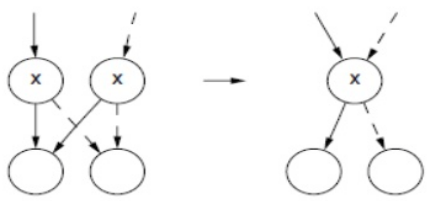
\includegraphics[scale=0.35]{slike/pravilo_spajanja.PNG}
    \caption{Pravilo spajanja}
    \label{fig:reductionRule}
\end{figure}

\begin{figure}[H]
    \centering
    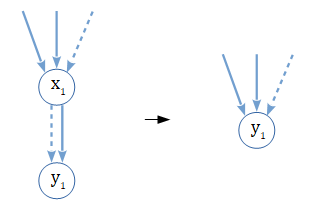
\includegraphics[scale=0.35]{slike/pravilo_eliminacije.PNG}
    \caption{Pravilo eliminacije}
    \label{fig:eliminationRule}
\end{figure}

Mana naivnog pristupa konstrukciji ROBDD je \v{s}to je on uvek eksponencijalne slo\v{z}enosti. Razlog za to je \v{s}to je kostrukcija kompletnog binarnog drveta odlu\v{c}ivanja skupa operacija, koja, pored velike vremenske slo\v{z}enosti, zauzima i eksponencijalno veliku koli\v{c}inu memorije u odnosu na broj promenljivih u ulaznoj formuli.

\begin{exmp}
    TODO
    Kada uradimo redukciju u programcicu, mozemo da ubazimo slicice
\end{exmp}


\subsubsection{Optimalna konstrukcija ROBDD}
\label{subsubsec:optimalROBDDConstruction}

Drugi na\v{c}in na koji je mogu\'c{}e konstruisati ROBDD takodje ima eksponencijalnu slo\v{z}enost. Medjutim, u praksi on daje dobre rezultate. Za razliku od prethodne metode, preska\v{c}e se medjukorak generisanja binarnog uredjenog drveta odlu\v{c}ivanja. Ovo dovodi do smanjenja potrebne memorije za njegovo generisanje, kao i do zna\v{c}ajnog ubrzanja algoritma.

Postupak je rekurzivan: kre\'c{}e se od bulovske funkcije koja se podeli na podfunkcije za koje se najpre generise ROBDD. Naredni korak je spajanje ove dve funkcije u jednu, uz kori\v{s}\'c{}enje pravila eliminacije i spajanja koja su opisana u prethodnoj sekciji.

Naredni primer oslikava efikasnu metodu za generisanje ROBDD.

\begin{exmp}
    TODO
\end{exmp}



